\subsection{Mikrocontroller}\label{subsec: Mikrocontroller}
Für die Auswahl des Mikrocontrollers, welcher auf dem Sensor wie auch auf dem Aktor-Layout eingebaut wird, werden die nachfolgenden Kriterien in Betracht bezogen. Das erste Kriterium ist die Rechenleistung des Controllers, welche die Aufgaben wie Kommunikation, ADC Wandlungen und einer kleine State Maschine übernehmen muss.
Ein weiteres Kriterium ist die Sicherheit, der Mikrocontroller soll den Benutzer schützen, darf somit keinen ungewollten Fremdzugriff auf vorhandene Daten wie auch auf Handlungen oder Schaltvorgänge zulassen. Ein weiteres Kriterium sind die Schnittstellen, welche die Funkverbindung zur Übertragung der Daten während des Betriebes gewährleisten, wie auch die Schnittstelle, bei welcher zu Beginn das Framework geladen wird. Das Pinout des jeweiligen Mikrocontrollers wird in den Unterkapiteln \ref{Hardware Mikrocontroller_Sensor} und \ref{Hardware Mikrocontroller_Aktor} besprochen. Bei der Auswahl wird als letztes Kriterium darauf geachtet, dass die Kosten für den Mikrocontroller nicht wahnsinnig hoch anfallen, sodass sich die Gesamtkosten des Systems in einem Rahmen befindet für eine mögliche Massenproduktion. Die fertig entwickelten Komponenten sollen sich zu einem Konkurrenzfähigem Preis verkaufen lassen.
\newpage
\subsection{Recherche}\label{subsec: Recherche}
Es wurden zwei geeignete Mikrocontroller miteinander verglichen, ihre Eigenschaften beschrieben und ausgewertet. 

\subsubsection{ESP32}
Der Mikrocontroller von der chinesischen Firma Espressif Systems ist ein Robuster Chip, welcher für industrielle Umgebungen geeignet ist und in Betriebstemperaturen von -40 °C bis +125 °C zuverlässig arbeitet. Der Stromverbrauch kann zwischen verschiedenen Leistungsmodi gewählt werden, so kann während dem Betrieb eine dynamische Leistungsskalierung bewerkstelligt werden. ESP32 Module sind mit integrierten Antennen, Leistungsverstärkern und rauscharmen Empfangsverstärkern hochintegriert. Schnittstellen wie SPI, I2C, UART, WiFi und Bluetooth sind vorhanden

\begin{figure}[H]
	\centering
	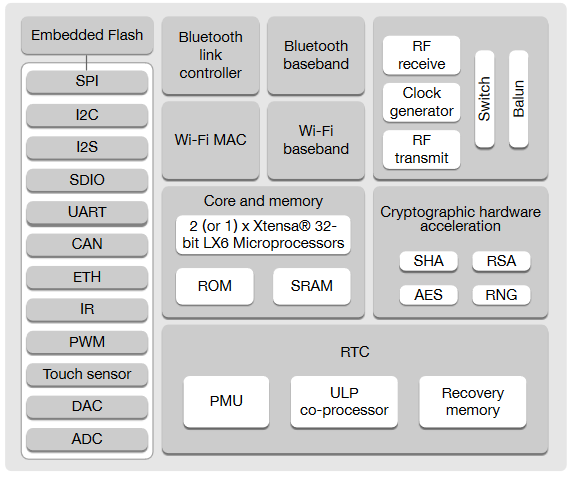
\includegraphics[width=\textwidth]{graphics/blockdiagrammESP32.PNG}
	\caption{Blockdiagramm ESP32 \cite{espressif_esp32-wroom-32_datasheet_en_2019}}
	
	\label{pic: blockdiagrammESP32}
\end{figure} 

WiFi:
Arbeitet mit dem Standart 802.11b/g/n und 802.11 2,4 GHz bis zu 150 Mbit/s. 4 Virtuelle Wi-Fi interfaces und Soft AP \\
\\
Bluetooth:
Kompatibel mit Bluetooth v4.2 BR/EDR und BLE-Spezifikationen. Sender Klasse 1, Klasse 2 und Klasse 3 ohne externen Leistungsverstärker. Hochgeschwindigkeits-UART HCI, bis zu 4 Mbits/s.\\
\\
CPU und Memory:
Modell abhängig, wobei das Modell ESP-WROOM-32E, mit der Chip Bezeichnung D0WD -V3 betrachtet wird. Dual-Core 32-bit, Flash 4-16 MB, 448 KB ROM, 520 KB SRAM, 16 KB SRAM in RTC. \\
\\
Prozessor:
Tensilica Xtensa LX6 240 MHz
\\
Clocks und Timers:
Interner 8 MHz-Oszillator mit Kalibrierung. Externer Quarzoszillator 2 MHz bis 40 MHz. Zwei Timer Gruppen 2x 64-bit Timer mit je einem Haupt Watchdog.\\
\\
Erweiterte Peripherieschnittstellen:
12-bit SAR ADC bis zu 18 Kanäle, 2x b-bit D/A Wandler, 10x touch Sensoren, Temperatursensor, 4x SPI, 2x I2S, 2x I2C 3x UART.\\
\\
Sicherheit:
Alle unterstützten Sicherheitsfunktionen des IEEE 802.11-Standards, einschließlich WFA, WPA/WPA2 und WAPI\\
\\
Unterstützung bei der Entwicklung:
SDK Firmware für schnelle on-line Programmierung und open Source toolchains basiert auf GCC.\\
\\
Kosten bei Mouser:
356-ESP32WROOM-32D 3,71 CHF/Stück
\newpage
\subsubsection{CC3235}
 Der CC3235 Controller ist eine Singel Chip Lösung von der Firma Texas Instruments. Dieser Chip ist mit einem Arm Cortex M4 MCU ausgestattet. Der CC3235 arbeitet un einer Industrieller Umgebung von -40 °C bis 85 °C zuverlässig. Schnittstellen wie UART, I2S, I2C, SPI und I/O Pins sind inbegriffen.

\begin{figure}[H]
	\centering
	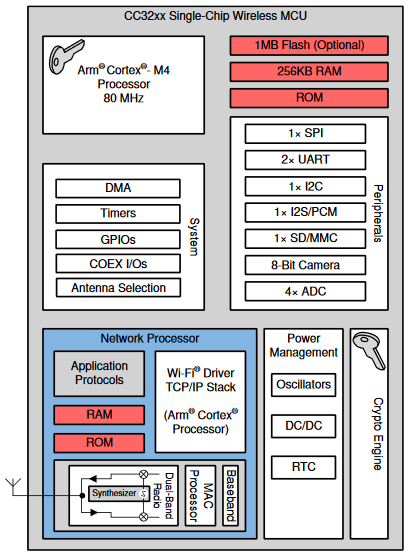
\includegraphics[width=0.75\textwidth]{graphics/blockdiagrammCC3235.PNG}
	\caption{Blockdiagramm CC3235 \cite{noauthor_cc3235s.pdf_nodate}}
	
	\label{pic: blockdiagrammCC3235}
\end{figure} 

WiFi: Arbeitet mit dem Standart 802.11 a/b/g/n 2.4 GHz und 5 GHz. Mit dem Netzwerkprozessor ist ein AP, Station(STA) sowie WiFi Direct Client inbegriffen.\\
\\
Bluetooth:
Der CC3235x ist für die Unterstützung von BLE/2,4 Funkkoexistenz ausgelegt\\
\\
CPU und Memory: Modell abhängig bei Betrachtung des Model CC3235SF, 1 MB Flash, 256 KB RAM. Ein 32-bit Arm Cortex-M4 Prozessor \\
\\
Prozessor: Arm Cortex-M4\\
\\
Clocks und Timer:
Interner 40 MHz Kristal Oszillator, 32,768 kHz  
Das Generalpurposetimermodule (GPTM) enthält 16- oder 32-Bit-GPTM-Blöcke. Jeder 16-  oder 32-Bit Block stellt zwei 16-bit Timer oder Zähler bereit.\\
\\
Erweiterte Peripherieschnittstellen:
1x SPI, 2x UART, 1x I2C, 1x i2s, 1x SD, 8-Bit Camera, 4x 12-bit ADC und 27 I/O Pins.\\
\\
Sicherheit:
Netzwerk-Passwörter und Zertifikate sind verschlüsselt und signiert. WEP, WPA /WPA2 PSK, WPA2 Enterpriese, WPA3 Personal.\\
\\
Unterstützung bei der Entwicklung:
CCS Uniflash ist das Standartwerkzeug zur Programierung von Texas Instruments MCU.

Kosten bei Mouser:
CC3235SF12RGKR 12.91 CHF/Stück

\subsection{Wahl des MCU}
 
 Im Kapitel \ref{subsec: Recherche} sind zwei geeignete MCU für diese Projekt gefunden worden. Im Vergleich zwischen dem CC3235 und dem ESP32 hat sich herausgestellt, dass der ESP32 preislich im Vorteil liegt und je nach Modul mit integrierter Antenne und oder SMA Anschluss angeboten wird. Somit fällt die Wahl auf den ESP32 der Firma Espressif Systems.
